\documentclass{standalone}

\usepackage[utf8]{inputenc}
\usepackage{tikz}

\begin{document}

% first method
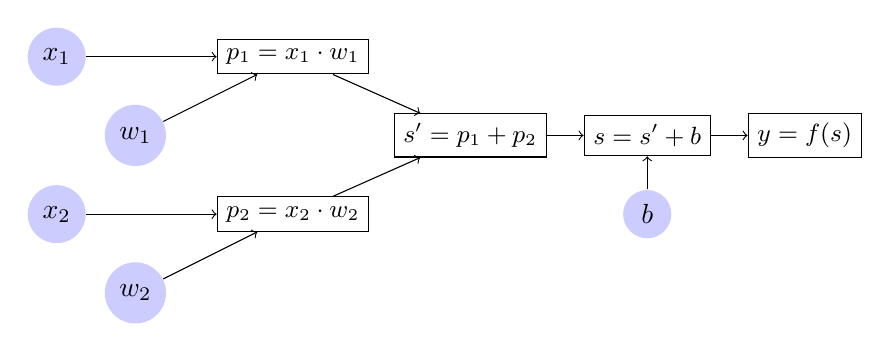
\begin{tikzpicture}[auto, node distance=3cm,
                    node_style/.style={circle,fill=blue!20},
                    edge_style/.style={->, draw=black},
                    sq/.style={draw, font=\small}
   ]
   \node[node_style] (x2) at (0,0) {$x_2$};
   \node[node_style] (x1) at (0,2) {$x_1$};
   \node[node_style] (w2) at (1,-1) {$w_2$};
   \node[node_style] (w1) at (1,1) {$w_1$};
   \node[node_style] (b) at (7.5, 0) {$b$};
   % Operations
   \node[sq] (p2) at (3,0) {$p_2 = x_2 \cdot w_2$};
   \node[sq] (p1) at (3,2) {$p_1 = x_1 \cdot w_1$};
   \node[sq] (sp) at (5.25,1) {$s' = p_1 + p_2$};
   \node[sq] (s) at (7.5,1) {$s = s' + b$};
   \node[sq] (y) at (9.5,1) {$y = f(s)$};

    \draw[edge_style]  (x1) edge node{} (p1);
    \draw[edge_style]  (w1) edge node{} (p1);
    \draw[edge_style]  (x2) edge node{} (p2);
    \draw[edge_style]  (w2) edge node{} (p2);
    \draw[edge_style]  (p1) edge node{} (sp);
    \draw[edge_style]  (p2) edge node{} (sp);
    \draw[edge_style]  (b) edge node{} (s);
    \draw[edge_style]  (sp) edge node{} (s);
    \draw[edge_style]  (s) edge node{} (y);
    \end{tikzpicture}
\end{document}
